\chapter{Orbital Stability and Transverse Linearization}
\label{ch:orbital_stability}

\section{Choose the Error That Matches the Task}

A swing can follow a similar spatial path at a different speed, arrive at
impact at a different time, or deliver a different face orientation at the
same time. These are different perturbations. Their importance depends on
the task and on which variables the path contains. A configuration path
omits velocity; a mechanical state-space path includes it. Sliding along
the latter is therefore not permission to choose an arbitrary speed along
the former. The compatibility conditions from Chapter 1 still apply.

Timed tracking compares $x(t)$ with a feasible reference $x_d(t)$ at the same
clock time. Orbital analysis compares a state with an invariant trajectory
set. Event-based analysis compares outcomes when a specified event occurs.
All three can be useful. A stationary ball may make some absolute start-time
shifts irrelevant, while clubhead speed, face orientation, contact order,
and timing relative to an external disturbance remain consequential. The
choice should follow the outcome, not a general preference for or against
time-indexed error.

Lyapunov stability means that sufficiently small initial perturbations remain
small. Asymptotic stability additionally requires convergence; exponential
stability specifies a rate bound. Lyapunov functions can analyze equilibria,
time-varying tracking errors, invariant sets, and periodic orbits. Orbital
stability is not an alternative that invalidates Lyapunov analysis. It is a
choice of the set whose stability we want to study.

For the unit-speed circle $x_d(t)=(\cos t,\sin t)$, a phase-shifted solution
$x_d(t-\varepsilon)$ has same-time distance
\begin{equation}\label{eq:timing_error}
 \|x_d(t-\varepsilon)-x_d(t)\|=2|\sin(\varepsilon/2)|.
\end{equation}
This remains small with small $\varepsilon$ and does not decay. It disproves
asymptotic convergence to the scheduled solution, not stability. For a system
driven by an explicit clock-dependent input, the shifted curve is not generally
a solution under the original input. Either shift the input too, use a
phase-dependent autonomous feedback law, or include the forcing phase in the
state before drawing an orbital conclusion.

\section{Invariant Orbits and Finite Segments}

Consider a smooth autonomous closed-loop system $\dot x=F(x)$ with a regular
nonstationary periodic solution $\gamma(t+T)=\gamma(t)$ of minimal period $T$.
Its image $\mathcal O$ is an invariant closed curve. In a neighborhood with a
specified distance, orbital stability means
\begin{equation}\label{eq:orbital_stability}
 \forall\epsilon>0\ \exists\delta>0:\quad
 d(x_0,\mathcal O)<\delta\ \Longrightarrow
 d(x(t),\mathcal O)<\epsilon\quad\text{for all }t\geq0.
\end{equation}
Asymptotic orbital stability adds $d(x(t),\mathcal O)\to0$ locally. Asymptotic
phase additionally means convergence to a particular time-shifted nominal
solution, $\|x(t)-\gamma(t+\theta_*)\|\to0$. These statements require the
relevant existence, invariance, and neighborhood conditions; they are not
inferred from a visually closed plot of a few coordinates.

A finite downswing segment is generally not invariant: its nominal solution
leaves through the endpoint. It cannot satisfy an all-future-time set-stability
definition merely because nearby motions remain close until impact. Useful
finite-horizon questions instead concern error amplification, constraint
satisfaction, disturbance sensitivity, and event outcomes before termination.
They need their own bounds. Calling a finite segment an orbit for descriptive
purposes should not transfer infinite-time theorems to it.

A nonstationary smooth periodic orbit is regular because its autonomous flow
cannot pass through an equilibrium and then leave under uniqueness. Arbitrary
reference curves can have stops, self-intersections, or endpoints. A projection
into selected measurements can intersect itself even if the full state orbit
does not. The state, metric, regularity, and selected phase neighborhood must
therefore be specified before constructing transverse coordinates.

The Van der Pol oscillator has an attracting limit cycle for positive damping
parameter in its standard form. It is a useful mathematical example. Walking
is often modeled with hybrid periodic gaits, and a golf swing is usually modeled
as a transient. Neither an analogy with an oscillator nor an attractive orbit
in a reduced model establishes a measured human coordination strategy.

\section{Derive the Local Phase and Transverse Coordinates}

Work first in a fixed Euclidean state chart with declared scaling. Let
$\gamma(\tau)$ be a regular reference, parameterized by its nominal physical
time $\tau$, and let $u_*(\tau)$ satisfy
$\gamma'(\tau)=f(\gamma(\tau),u_*(\tau))$. Define
$v(\tau)=\|\gamma'(\tau)\|>0$, unit tangent $T=\gamma'/v$, and a smooth
orthonormal normal basis $E(\tau)\in\mathbb R^{n\times(n-1)}$, with
$E^TE=I$ and $E^TT=0$. A local coordinate representation is
\begin{equation}\label{eq:decomposition}
 x=\gamma(\tau)+E(\tau)\xi,\qquad \xi\in\mathbb R^{n-1}.
\end{equation}
The ambient displacement $E\xi$ has $n$ components; the reduced error $\xi$
has $n-1$. The orthogonal projector $P=EE^T=I-TT^T$ is an $n\times n$
matrix. Projecting with $P$ does not itself produce reduced coordinates.

For nearest-point phase, $T(\tau)^T[x-\gamma(\tau)]=0$. This defines a smooth
local phase only where its derivative with respect to $\tau$ is nonzero and
the chosen closest point is unique. A compact embedded curve has an appropriate
tubular neighborhood, but a curvature radius alone does not establish its
global width: distant pieces of the curve can approach one another. Endpoints
and branch changes need explicit handling. Frenet frames can fail at zero
curvature; a smooth normal frame can often be constructed without that failure.

Differentiate the coordinate representation and project along $T$ and $E$.
For $u=u_*(\tau)+\delta u$, the exact local equations are
\begin{equation}\label{eq:orbital_exact_transverse}
 \dot\tau=\frac{T^Tf(x,u)}{v-T'^TE\xi},\qquad
 \dot\xi=E^Tf(x,u)-E^TE'\xi\dot\tau.
\end{equation}
Primes here mean derivatives with respect to nominal time $\tau$, and dots
mean actual physical time. We used $T^TE'=-T'^TE$. The denominator must remain
nonzero; forward progression additionally requires $\dot\tau>0$. At the
reference $\dot\tau=1$ and $\dot\xi=0$. This is the nominal-time version of
Chapter 2's arc-length equations, with its parameter factors made explicit.

Linearization at fixed phase gives
\begin{equation}\label{eq:transverse_linear}
 \dot\xi=A_\perp(\tau)\xi+B_\perp(\tau)\delta u
       +O(\|\xi\|^2+\|\delta u\|^2),
\end{equation}
\begin{equation}\label{eq:transverse_practical}
 A_\perp=E^Tf_xE-E^TE',\qquad B_\perp=E^Tf_u.
\end{equation}
Mixed second-order terms are absorbed into the displayed bound locally.
The dimensions are $(n-1)\times(n-1)$ and $(n-1)\times m$, respectively.
The frame derivative matters; an arbitrary sequence of independently computed
normal bases can introduce sign jumps and fictitious dynamics. In a rotating
normal basis this term transforms with the basis, preserving the physical
prediction when the full transformation is retained.

The derivation assumes an autonomous plant and feedforward evaluated at the
estimated phase. Explicit time dependence, an independent clock-driven input,
or a dynamic phase estimator adds variables or coupling terms. For a manifold
state use compatible local charts, connections, or group coordinates as in
Chapter 3. The fixed-chart formula should not be applied unchanged to an
arbitrary position-dependent metric. Under a different path parameter, both
the speed and cost integration measure must be transformed consistently.

\subsection{An Oscillator With a Missing Input Factor}

For $\dot x_1=x_2$, $\dot x_2=-x_1+u$, take
$\gamma(\tau)=(\cos\tau,-\sin\tau)$ and $u_*=0$. Then
$T=(-\sin\tau,-\cos\tau)^T$, $E=(-\cos\tau,\sin\tau)^T$, and
$x=(1-\xi)\gamma(\tau)$. The equations become
\begin{equation}\label{eq:orbital_oscillator}
 \dot\xi=u\sin\tau,\qquad
 \dot\tau=1-\frac{u\cos\tau}{1-\xi},\qquad
 A_\perp=0,\quad B_\perp=\sin\tau.
\end{equation}
Choose $u=-k\sin\tau\,\xi$ with $k>0$. The exact radial equation is
$\dot\xi=-k\sin^2\tau\,\xi$; along the nominal orbit $\tau=t$ its scalar
linearization has one-period multiplier
\begin{equation}\label{eq:orbital_oscillator_multiplier}
 \mu=\exp\!\left(-k\int_0^{2\pi}\sin^2t\,dt\right)=e^{-k\pi}<1.
\end{equation}
This is a local exponential-stability certificate with the usual smoothness
and regular-phase assumptions. No averaging is required for the multiplier.
The incorrect law $u=-k\xi$ instead gives exponent
$-k\int_0^{2\pi}\sin t\,dt=0$ and multiplier one. The missing sine factor
changes the conclusion. For sufficiently small $\xi$, forward phase remains
well-defined; this local argument does not establish global behavior at the
origin, where radial phase is undefined, or under torque saturation.

The related exercise $\dot x_1=x_2+u$, $\dot x_2=-x_1^3$ cannot track the
same timed circle by any choice of $u$: the second equation would require
$-\cos t=-\cos^3t$ for all $t$. Checking the uncontrolled equation should
precede linearization, optimization, or feedback design.

\section{What Linearization Can Certify}

For a smooth invariant orbit, uniform exponential stability of the transverse
linearization implies local exponential orbital stability under standard
regularity conditions. An unstable transverse multiplier gives local
instability. A marginal linearization generally leaves nonlinear behavior
undecided. Nonlinear asymptotic stability is not equivalent to asymptotic
stability of the linearized system.

For example, in a local annulus use angular phase $\dot\theta=1$ and radial
error dynamics either $\dot\xi=-\xi^3$ or $\dot\xi=+\xi^3$. Both have the
same circle and the same transverse linearization $\dot\xi=0$. Yet
\begin{equation}\label{eq:orbital_nonlinear_marginal}
 \xi_-(t)=\frac{\xi_0}{\sqrt{1+2\xi_0^2t}},\qquad
 \xi_+(t)=\frac{\xi_0}{\sqrt{1-2\xi_0^2t}}.
\end{equation}
The first converges algebraically; the second grows until it leaves the local
region. Both linearizations have multiplier one. Higher-order terms decide
the distinction. This counterexample also explains why a linear Lyapunov
function is a candidate for nonlinear verification, not an automatic proof
over a large tube.

\section{Periodic Orbits, Return Maps, and Hybrid Events}

For a periodic transverse linear system $\dot\xi=A_\perp(t)\xi$, the state
transition matrix satisfies $\partial_t\Phi(t,t_0)=A_\perp(t)\Phi(t,t_0)$,
$\Phi(t_0,t_0)=I$. Its one-period map $M_\perp=\Phi(T,0)$ has Floquet
multipliers as eigenvalues. All magnitudes strictly below one give exponential
stability of this periodic linear system and local exponential stability of
the smooth nonlinear orbit. Any magnitude above one implies instability.
For the linear system, semisimple unit-modulus multipliers can permit bounded
solutions; for the nonlinear orbit they are inconclusive without more analysis.

A nonstationary autonomous periodic orbit has a unit multiplier in the full
variational system because its tangent is a periodic solution of that system.
There may be additional unit multipliers. Transverse reduction removes the
phase direction, not every possible neutral mode. Periodically forced systems
do not automatically have the same neutral phase direction when the forcing
clock is held fixed. An augmented phase formulation must state what is varied.

A local Poincare section crosses the flow transversely near a point on a
periodic orbit. The local return map has a fixed point there. Its derivative
represents the transverse monodromy map up to a consistent change of section
coordinates; numerical matrices need not be literally equal under different
bases. Their nontrivial multipliers agree. A phase basis used around a cycle
must also be identified consistently after one period; a frame mismatch can
alter an incorrectly assembled return matrix.

A hypothetical return map with diagonal multipliers $0.7,0.4,-0.3$ contracts
those eigenmodes, with the last alternating sign. Along the first eigenmode,
ten returns give factor $0.7^{10}\approx0.028$. This is an illustrative map,
not a computed walking or golf result. Nonnormal eigenvectors can produce
large norm growth before asymptotic decay. A gain that moves a multiplier
cannot be computed from the multiplier alone: the input map is required.
For $z_{j+1}=1.1z_j+b u_j$, $u_j=-kz_j$, the target $0.6$ requires
$k=0.5/b$ when $b\ne0$.

Hybrid motion requires the event and reset derivative as well as continuous
variational integration. For a smooth guard $h(x,t)=0$, reset
$x^+=\Delta(x^-,t)$, and transverse crossing
$h_t+h_xf^-\ne0$, the saltation matrix mapping perturbations at a common
nominal time is
\begin{equation}\label{eq:orbital_saltation}
 S=\Delta_x+
 \frac{(f^+-\Delta_x f^--\Delta_t)h_x}{h_t+h_xf^-}.
\end{equation}
This includes the effect of changed event time. A hybrid cycle's linear map
composes continuous transitions and these event maps in chronological order,
with consistent coordinates. Grazing, simultaneous contacts, or changes in
event order can invalidate this smooth local formula.

Even an identity reset does not imply $S=I$. In one dimension, let speed
change from one to two when $x$ crosses zero. Then $S=2$: a small position
lead triggers the faster mode earlier and doubles the subsequent position
lead. Differentiating only the identity reset would miss this effect.
Club-ball contact, ground contact, and changing grip constraints likewise
need a stated event model; a smooth downswing Jacobian alone does not
describe sensitivity across an impact.

\section{Finite-Time Amplification and Impact Sensitivity}

For a transient, $\Phi(t_2,t_1)$ gives first-order sensitivity under its stated
closed-loop dynamics. In a fixed Euclidean norm its largest singular value
is a worst-case amplification factor. A value above one means \emph{some}
initial direction is amplified, not all directions. A terminal value below
one does not exclude earlier growth. Higher-order errors and ongoing
disturbances also remain outside that homogeneous linear map.

The stable constant matrix
\begin{equation}\label{eq:orbital_transient_growth}
 A=\begin{pmatrix}-1&10\\0&-1\end{pmatrix},\qquad
 \Phi(t,0)=e^{-t}\begin{pmatrix}1&10t\\0&1\end{pmatrix}
\end{equation}
has both eigenvalues at $-1$. Nevertheless $\|\Phi(1,0)\|_2>3.7$, while
$\|\Phi(10,0)\|_2<0.005$. A small final error does not prove an intermediate
joint or contact constraint was respected. Bounds should cover the whole
relevant interval and the actual output, not just a terminal state norm.

With positive-definite endpoint metrics $W_1,W_2$, the consistent gain is
\begin{equation}\label{eq:amplification}
 \rho_W=\|W_2^{1/2}\Phi(t_2,t_1)W_1^{-1/2}\|_2.
\end{equation}
Changing coordinate units without transforming the metrics changes the
numerical gain and can change whether it exceeds one. Output sensitivity
may matter more than the norm of the full transverse state: some directions
barely affect face orientation, while others have large task consequences.
For phase-to-phase integration, convert $d\xi/dt$ to $d\xi/ds$ with the
phase rate; do not substitute a path coordinate for time in an unchanged ODE.

Impact is usually an event rather than a fixed clock time. Let the nominal
event occur at $t_e$, with $a=h_t+h_xf\ne0$ and a pre-event fixed-time
perturbation $\delta x=\Phi(t_e,t_0)\delta x_0$. To first order,
\begin{equation}\label{eq:orbital_event_sensitivity}
 \delta t_e=-\frac{h_x\delta x}{a},\qquad
 \delta x_e=\delta x+f\delta t_e,\qquad
 \delta y=H_x\delta x+(H_xf+H_t)\delta t_e.
\end{equation}
Here $y=H(x_e,t_e)$ is the event output, and all derivatives are evaluated
on the nominal pre-event state. A reset requires its own derivative afterward.
The denominator reveals why near-grazing events can have large timing
sensitivity even when fixed-time state perturbations look modest.

For constant-speed travel $\dot q=v$, $\dot v=0$ toward $q=L$, the fixed-time
transition is $\Phi=\left(\begin{smallmatrix}1&t_e\\0&1\end{smallmatrix}\right)$.
At the event, position perturbation is zero by definition, but velocity
perturbation remains and
$\delta t_e=-(\delta q_0+t_e\delta v_0)/v$. A metric that discards event
time is appropriate only if the task also discards it. A metric that discards
velocity would miss a central contributor to impact performance.

\section{LQR With the Correct Variables and Cost}

For the reduced linear model, define the finite-horizon cost
\begin{equation}\label{eq:orbital_lqr_cost}
 J=\xi(T)^TS_T\xi(T)+\int_0^T
       (\xi^TQ(t)\xi+\delta u^TR(t)\delta u)\,dt,
 \qquad Q,S_T\succeq0,\quad R\succ0.
\end{equation}
With appropriate continuous bounded coefficients and positive-definite $R$,
the finite-horizon Riccati solution gives
\begin{equation}\label{eq:riccati}
 -\dot S=A_\perp^TS+SA_\perp-SB_\perp R^{-1}B_\perp^TS+Q,
 \quad S(T)=S_T,\quad K=R^{-1}B_\perp^TS.
\end{equation}
The input law is
\begin{equation}\label{eq:full_control_law}
 u=u_*(\tau)-K(\tau)\xi,\qquad
 \xi=E(\tau)^T[x-\gamma(\tau)].
\end{equation}
Its correction has $m$ components. Multiplying $K\xi$ by the state basis
$E$ is generally dimensionally invalid: that basis maps reduced state error
to ambient state displacement, not to actuator input. The negative sign
follows the stated gain convention. Finite-horizon optimality for this linear
cost is not an unlimited-time stability theorem or a nonlinear optimum.

Evaluating a nominal-time gain schedule at measured phase creates a
phase-dependent controller. The exact dynamics include $\dot\tau$, so an
off-reference nonlinear certificate must differentiate $S(\tau)$ with that
actual rate. If the optimization itself uses another phase coordinate $s$,
then $dt=ds/\dot s$ changes the dynamics and running cost. A frozen nominal
conversion can be a local design approximation, but should not be described
as an exact nonlinear optimal-control solution.

The value $V=\xi^TS\xi$ satisfies
\begin{equation}\label{eq:orbital_lqr_dissipation}
 \dot V=-\xi^T(Q+K^TRK)\xi
\end{equation}
along the ideal linear closed loop. If $S>0$, a constant level set gives an
invariant time-varying ellipsoid for that linear system. Its axis radii are
$\sqrt{c/\lambda_i(S)}$, but they need not decrease toward the terminal time.
For a scalar integrator with $Q=R=1$, $T=1$, and $S_T=1/4$,
\begin{equation}\label{eq:orbital_riccati_counterexample}
 S(t)=\tanh(1-t+\operatorname{arctanh}(1/4)).
\end{equation}
This positive solution decreases toward $1/4$, so a fixed-level ellipsoid
expands. A larger terminal penalty or state weight does not by itself prove
monotone tightening, feasible torque, or improved impact variance. Those
claims require the resulting closed-loop and task calculations.

\begin{figure}[htbp]
\centering
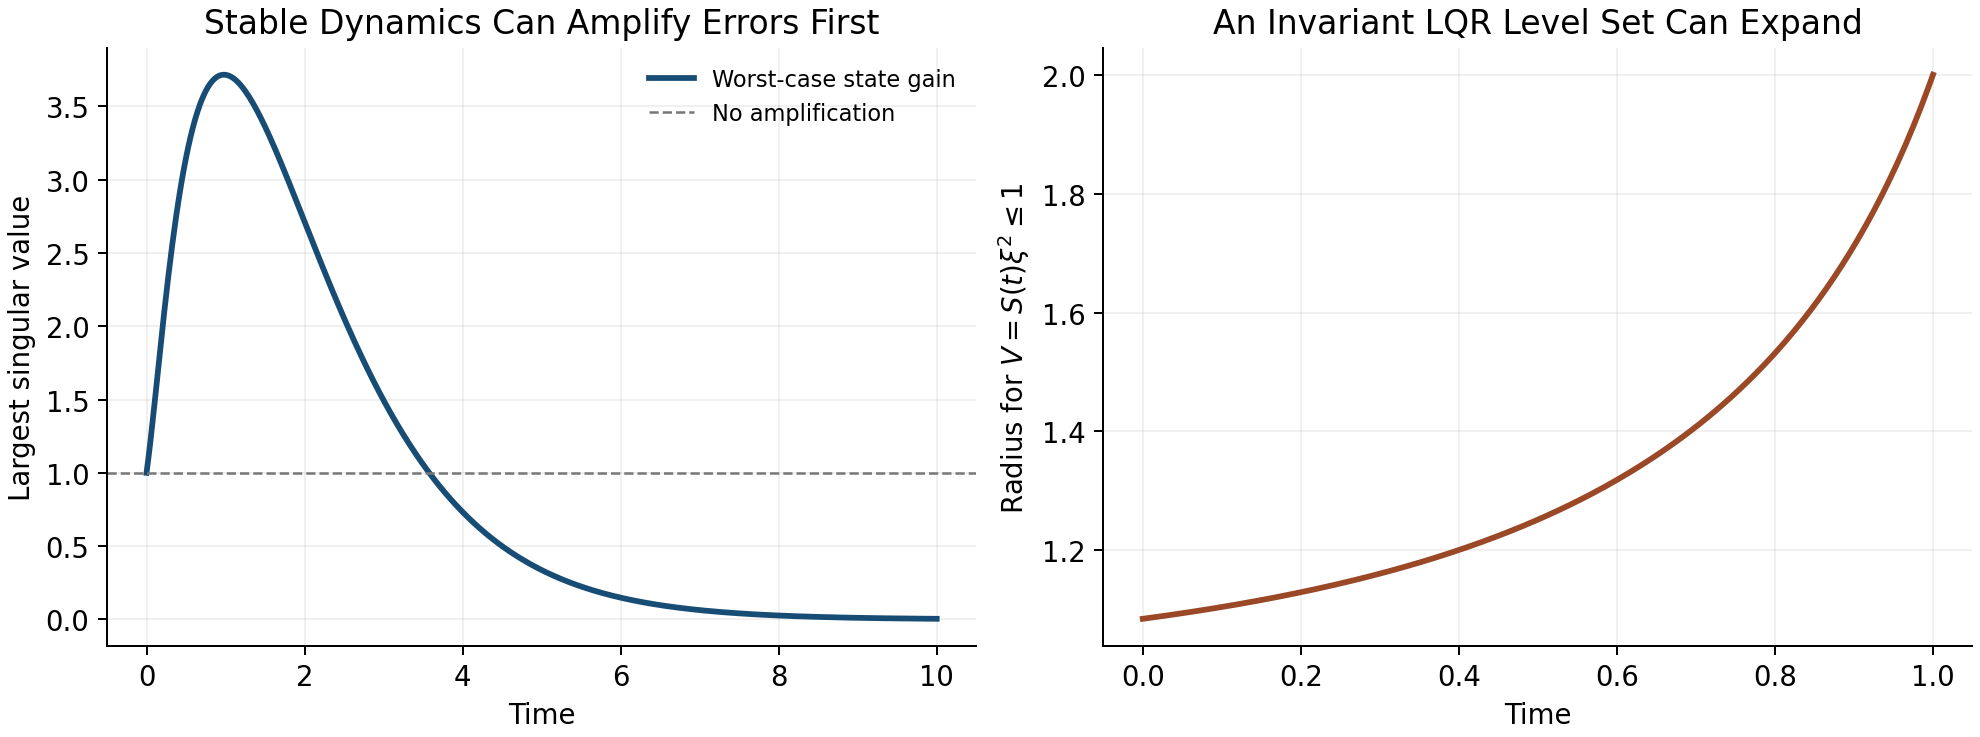
\includegraphics[width=\textwidth]{../figures/orbital_transient_bounds.png}
\caption{Transient Growth and Expanding Invariant Sets}
\label{fig:orbital_transient_bounds}
\end{figure}
The left panel evaluates the triangular transition matrix above; the right
evaluates the scalar Riccati radius with level one. Both are calculated
counterexamples, not measured golf profiles. Together they separate asymptotic
stability, intermediate amplification, and the geometric width of a verified set.

Standard full-state time-varying LQR can use nonuniform weights and explicitly
represent task-relevant directions. It does not inherently penalize all errors
equally. Transverse design is useful when phase freedom matches the task and
the phase estimate is reliable. Timed tracking is useful when schedule matters.
The comparison should use equal constraints, uncertainty assumptions, and
outcome criteria, rather than assume one architecture always expends less effort.

\section{Verify Nonlinear Tubes and Disturbance Effects}

For a candidate tube $V(\tau,\xi)\leq c(\tau)$, verify on its boundary
\begin{equation}\label{eq:orbital_tube_boundary}
 V_\tau\dot\tau+V_\xi\dot\xi\leq c'(\tau)\dot\tau
\end{equation}
under the actual nonlinear controller, admissible disturbances, and input
bounds, with the initial condition inside. Also verify phase-coordinate
validity, event ordering, and any reset inclusion into the next tube. A
positive Riccati matrix is a useful starting candidate, not a replacement
for these checks. For $\dot\xi=-\xi+\xi^3$, the quadratic $V=\xi^2$ has
$\dot V=-2\xi^2+2\xi^4$: the linearized dissipation holds locally but fails
outside $|\xi|=1$. Available actuator authority alone does not repair an
unverified nonlinear inequality.

For additive linear disturbances, the propagation is
\begin{equation}\label{eq:orbital_disturbance}
 \xi(t)=\Phi(t,0)\xi_0+
       \int_0^t\Phi(t,s)D(s)d(s)\,ds.
\end{equation}
Even strong attenuation of initial error does not eliminate disturbances
arriving near impact. For white-noise diffusion with covariance intensity
$Q_d$, a linear covariance model satisfies
$\dot\Sigma=A_{\rm cl}\Sigma+\Sigma A_{\rm cl}^T+DQ_dD^T$.
This is a stochastic-model assumption, not a universal description of motor
noise. Event-output covariance additionally uses the event sensitivity map,
and uncertainty in estimated phase or model parameters must be included.

Classical gain and phase margins concern specified frequency-domain loop
models under particular assumptions. An arbitrary time-varying transverse
system has no ordinary stationary transfer function to which those margins
can be assigned unchanged. Setting $R=rI$ in finite-horizon LQR does not
establish universal per-channel half-gain or sixty-degree margins for a
time-varying nonlinear swing controller. Appropriate alternatives include
verified Lyapunov inequalities over an uncertainty set, induced-gain bounds,
delay-aware models, and explicit perturbation studies. Simulation evidence
should be distinguished from a worst-case certificate.

\section{A Reproducible Golf Stability Investigation}

Define the measured state and the impact event first. State whether the
comparison is at common time, common phase, or each swing's own impact, and
which output coordinates determine success. Include clubhead velocity and
face orientation with their measurement uncertainties rather than treating
proximity in an arbitrary state plot as sufficient evidence of accuracy.

Next construct a feasible nominal motion and identify what is held fixed in
the perturbation experiment: prescribed torques, phase-dependent feedback,
an estimated biological controller, or a passive model. A nominal trajectory
does not identify its surrounding closed-loop vector field. Different
feedback laws can generate the same nominal swing and different stability.
Inverse dynamics supplies model-dependent net force requirements; it does
not alone reveal how those forces change after a perturbation.

Compute the variational dynamics, phase transformation, and event/reset maps
for that model. Test numerical derivatives against finite perturbations and
check convergence with integration tolerance and perturbation size. Examine
weighted singular values throughout the motion, not just eigenvalues or the
final gain. Propagate realistic ongoing disturbances and inspect input,
contact, and joint constraints. Estimate nonlinear validity by direct tests
or a certificate with a stated region.

Only then compare a proposed passive-assistance mechanism with a changed
model or controller. Recompute the trajectory and impact event under the
intervention. Report whether a difference comes from initial-error attenuation,
disturbance rejection, timing, output sensitivity, or altered nominal speed.
These aspects can interact: higher speed can improve a performance objective
while reducing correction time, and a stable state direction may have little
effect on the ball. There is no universal numerical amplification profile
through backswing, transition, release, and impact established by geometry alone.

Validate the predicted distinctions on held-out data and report alternative
models that fit equally well. A reduction in a model's transverse norm is
evidence about that model and metric. Calling it improved repeatability requires
the event-output distribution; attributing it to human feedback requires
additional identification or intervention evidence. Feedforward and feedback
contributions should be measured under a stated decomposition, not assigned
a fixed ninety-to-ten percentage.

\section{Further Reading}

\href{https://underactuated.mit.edu/limit_cycles.html}{Tedrake's limit-cycle
notes} and \href{https://underactuated.mit.edu/lqr.html}{LQR treatment} explain
trajectory and orbital analysis within Lyapunov and optimal-control methods.
\href{https://arxiv.org/abs/1010.2241}{Manchester's transverse-dynamics work}
develops local coordinates and nonlinear region verification.
\href{https://arxiv.org/abs/2306.06862}{Kong and colleagues' saltation tutorial}
explains event-time corrections in hybrid linearization. Their assumptions
must be matched to the swing model before transferring a stability conclusion.

\section{Exercises}

\begin{enumerate}[itemsep=3pt,parsep=0pt]
\item Compute the same-time distance between two phase-shifted unit circles.
Distinguish bounded error, convergence to the scheduled solution, and orbital
convergence. Explain what changes with a fixed periodic forcing clock.
\item Derive the nominal-time phase and reduced equations from
$x=\gamma(\tau)+E(\tau)\xi$. State matrix dimensions and the denominator
condition. Convert to an arc-length parameter and check the speed factors.
\item Verify the oscillator's two feedback laws and their linear multipliers.
Simulate small radial perturbations and compare with $e^{-k\pi}$ after one
cycle. Check phase positivity and input saturation separately.
\item Compare $\dot\xi=-\xi^3$ and $\dot\xi=+\xi^3$ around a periodic orbit.
Explain why their identical unit multiplier does not settle nonlinear stability.
\item Test feasibility of the proposed circle in
$\dot x_1=x_2+u$, $\dot x_2=-x_1^3$. Identify the violated equation before
attempting a feedback or optimization calculation.
\item Compute singular values of the triangular transition matrix throughout
$0\leq t\leq10$. Compare transient gain with its eigenvalues, then repeat
after coordinate scaling with and without transforming the metric.
\item Derive the event-time and output sensitivity for constant-speed travel.
Check it by finite differences, then add an identity-reset speed switch and
verify the saltation factor two.
\item Verify the scalar Riccati solution with terminal weight $1/4$ and plot
the fixed-level radius. Explain how invariance and expanding geometric width
can coexist. Test the nonlinear cubic remainder on a candidate tube.
\item For $z_{j+1}=1.1z_j+b u_j$, compute gains producing multiplier $0.6$
for $b=1$ and $b=2$. Explain why multiplier data alone cannot determine a gain.
\item Design a model-based swing experiment separating initial-error reduction,
ongoing noise, phase uncertainty, and impact-output sensitivity. Specify an
intervention and held-out evidence that would distinguish competing explanations.
\end{enumerate}
